\section{Introduction}

This paper deals with the problem of the worst-case time complexity estimations for relational programs in \mK. Despite its simple implementation, the search in \mK has a number of subtleties
affecting the performance which are hard to think about intuitively altogether. It is easy to overlook some of them and the behavior of the search in certain cases can be really surprising.

\begin{figure}[t]
\begin{tabular}{p{5cm}p{5cm}}
\begin{lstlisting}[basicstyle=\small]
   length$^o$ = fun a n ->
     ((a === Nil) /\ (n === O)) \/
     (fresh (h t n')
        (a === Cons (h, t)) /\
        (n === S (n')) /\
        (length$^o$ l' n'))
     )
\end{lstlisting} &
\begin{lstlisting}[basicstyle=\small]
   length$_d^o$ = fun a n ->
     ((a === Nil) /\ (n === O)) \/
     (fresh (h t n')
        (a === Cons (h, t)) /\
        (length$_d^o$ l' n') /\
        (n === S (n')))
     )
\end{lstlisting}
\end{tabular}
\caption{Example of two implementations of the length calculating relation}
\label{fig:length_implementations}
\end{figure}

\begin{figure}[t]
    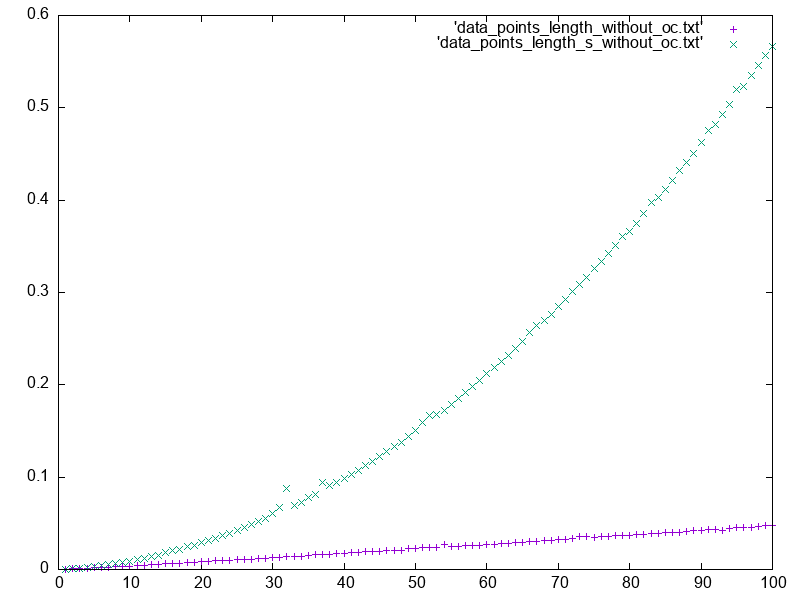
\includegraphics[width=6cm,height=5cm]{lengths_without_oc.png}
    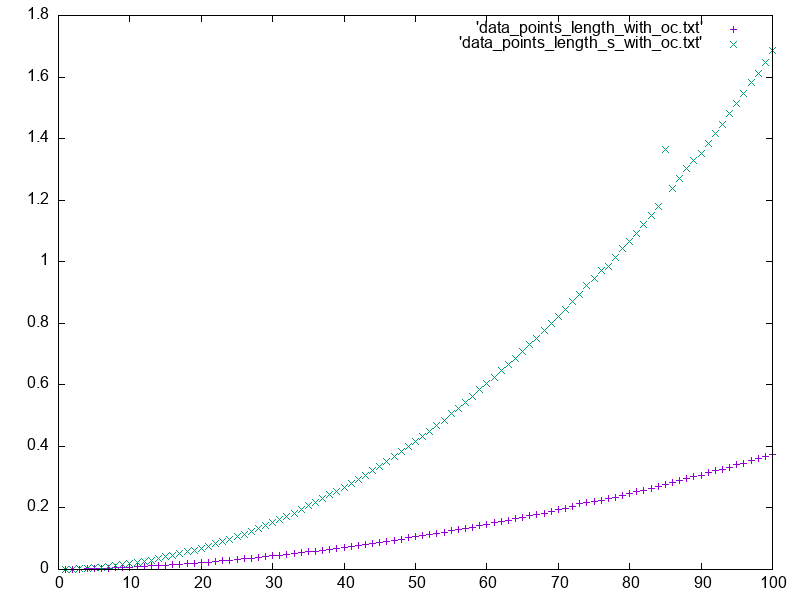
\includegraphics[width=6cm,height=5cm]{lengths_with_oc.png}
  \caption{Time of the search for the relations \lstinline|length$^o$| (purple) and \lstinline|length$_d^o$|} (green).
  Left: without occurs check.
  Right: with occurs check.
  \label{fig:length_plots}
\end{figure}

As a motivative example, consider two implementations of a standard recursive relation calculating the length of a list (see \figureword~\ref{fig:length_implementations}). They differ only in the
orders of conjuncts. Although the \lstinline|length$_d^o$| relation can be seen as a more direct definition of a function as a relation (all steps of usual length evaluation written up in order),
it is well-known that the \lstinline|length$^o$| with the recursive call in the end is much faster when running this relation backward (in fact, the search diverges if we
run \lstinline|length$_d^o$| backward, while for \lstinline|length$^o$| it terminates). What is less known and what we find more unexpected is the fact that if we run both relation
forward (specifying the list and asking for the length) \lstinline|length$^o$| is still much faster than \lstinline|length$_d^o$|, although they perform the same number of unifications
(actually during the evaluation of \lstinline|length$^o$| unified terms are even bigger). You can see the comparative time of the search in \figureword~\ref{fig:length_plots}. The difference is even
more staggering if we switch off occurs checks in unifications (for simple queries like this occurs checks never violated). In the same \figureword~\ref{fig:length_plots} you can see that
the \emph{asymptotic complexity} becomes different in this case: it is linear for \lstinline|length$^o$| and quadratic for \lstinline|length$_d^o$|.

After investigating the execution for this example in detail we found that the difference is caused not by unifications but by the process of \emph{scheduling} of goals during the search.
During the execution of a program in \mK a lazy structure is build that decomposes the goals into unifications, performs these unifications in a certain order and passes the results
appropriately. In our example this structure becomes linear in size just because of the order in conjunctions (when the recursive call is not the last) and increases the time of
scheduling significantly. This kind of effects is hard to predict and measure without a formal model for performance in \mK.

This paper presents such a model. We state that the total time of the search in \mK breaks into three separate parts: the time of scheduling ($T_s$) that breaks the evaluation into a sequence of
unifications, the time required to perform these unifications, and the time of reifications ($T_r$) that reconstruct the result in an expected form in the end. The time of unifications can be further
divided into the time of occurs checks ($T_{occ}$) during the unification and the time ($T_{uni}$) of the rest of the unification algorithm (this division will help us to see how large
is the part of the total time that occurs check, which often can be ommited, takes). So the total time of the search can be calculated as the sum of four components:

\[ T = T_s + T_{uni} + T_{occ} + T_r \]

We show how these components can be estimated and compared to each other in terms of asymptotics. The scheduling time complexity can be measured precisely since we link it to a specific value which we
call \emph{scheduling factor}, defined in terms of existing formal semantics of \mK (we recall the existing formal descriptions of \mK in \sectionword~\ref{sec:background}) and can be calculated using
a number of equations (\sectionword~\ref{sec:scheduling}). The other time components are hard to estimate precisely in general, as they are connected to the unification process, but we identify two
criteria that determine a wide range of cases for which these time components can be estimated easily (\sectionword~\ref{sec:uni-rei}). These separate methods for estimation of
different components of the time of the search can be put together in one approach calculating the time complexity for a given query to a recursive relation (if this query satisfies the stated
criteria) using the principles of symbolic execution (\sectionword~\ref{sec:symbolic}). We then show the applicability of our method by applying it for a number of realistic \mK relations (\sectionword~\ref{sec:evaluation}).
